\documentclass{beamer}
\usepackage[T1]{fontenc}
\usepackage[utf8]{inputenc}
\usepackage{lmodern}
\usepackage{amsmath,amssymb,mathtools,bm}
\usepackage{booktabs,array,graphicx,listings,xcolor}
\usetheme{Boadilla}
\useoutertheme{miniframes}
\setbeamertemplate{navigation symbols}{}
\setbeamertemplate{itemize items}[default]
\definecolor{codeblue}{RGB}{42,55,150}
\definecolor{lecturekey}{RGB}{162,30,37}
\lstset{language=Python,basicstyle=\ttfamily\scriptsize,
  keywordstyle=\color{codeblue},showstringspaces=false,
  columns=fullflexible,keepspaces=true,frame=single,breaklines=true}
\newcommand{\keytext}[1]{\textcolor{lecturekey}{\textbf{#1}}}
\newcommand{\keybox}[1]{\textcolor{lecturekey}{\boxed{#1}}}
\newcommand{\E}{\mathbb E}
\newcommand{\Var}{\operatorname{Var}}
\newcommand{\Cov}{\operatorname{Cov}}
\newcommand{\SE}{\operatorname{SE}}
\newcommand{\pos}[1]{(#1)^+}
\newcommand{\redstar}{\textcolor{red}{*}}



\graphicspath{{figures/}}
\newcommand{\QOneStates}{6, 13, 14, 5, 6, 13, 14, 5, 6, 13, 14, 5, 6, 13, 14, 5, 6, 13, 14, 5}
\newcommand{\QOneUniforms}{0.3750, 0.8125, 0.8750, 0.3125, 0.3750, 0.8125, 0.8750, 0.3125, 0.3750, 0.8125, 0.8750, 0.3125, 0.3750, 0.8125, 0.8750, 0.3125, 0.3750, 0.8125, 0.8750, 0.3125}
\newcommand{\QTwoMean}{2.029487}
\newcommand{\QTwoVariance}{4.074184}
\newcommand{\QThreeProposals}{15100}
\newcommand{\QThreeEfficiency}{0.662252}
\newcommand{\QFourExact}{0.746824133}
\newcommand{\QFourAMean}{0.747220}
\newcommand{\QFourASD}{0.197787}
\newcommand{\QFourALow}{0.708454}
\newcommand{\QFourAHigh}{0.785986}
\newcommand{\QFourBMean}{0.746617}
\newcommand{\QFourBSD}{0.201933}
\newcommand{\QFourBLow}{0.734101}
\newcommand{\QFourBHigh}{0.759133}
\newcommand{\QFourCMean}{0.743719}
\newcommand{\QFourCSD}{0.201024}
\newcommand{\QFourCLow}{0.739779}
\newcommand{\QFourCHigh}{0.747659}
\newcommand{\QFourDMean}{0.746570}
\newcommand{\QFourDSD}{0.200986}
\newcommand{\QFourDLow}{0.745324}
\newcommand{\QFourDHigh}{0.747816}
\newcommand{\QFiveExact}{13.455050}
\newcommand{\QFiveAMean}{13.267172}
\newcommand{\QFiveASD}{26.497851}
\newcommand{\QFiveASE}{0.264979}
\newcommand{\QFiveALow}{12.747814}
\newcommand{\QFiveAHigh}{13.786529}
\newcommand{\QFiveBMean}{13.439328}
\newcommand{\QFiveBSD}{27.220361}
\newcommand{\QFiveBSE}{0.086078}
\newcommand{\QFiveBLow}{13.270615}
\newcommand{\QFiveBHigh}{13.608042}
\newcommand{\QSixAVMean}{13.646271}
\newcommand{\QSixAVSD}{16.678473}
\newcommand{\QSixAVSE}{0.166785}
\newcommand{\QSixAVLow}{13.319373}
\newcommand{\QSixAVHigh}{13.973169}
\newcommand{\QSixCrudeMean}{13.603578}
\newcommand{\QSixCrudeSD}{27.161508}
\newcommand{\QSixCrudeSE}{0.271615}
\newcommand{\QSixCrudeLow}{13.071212}
\newcommand{\QSixCrudeHigh}{14.135943}
\newcommand{\QSevenCoeff}{-0.863741}
\newcommand{\QSevenExact}{0.961766}
\newcommand{\QSevenExactCoeff}{-0.865589}
\newcommand{\QSevenCrudeMean}{0.985239}
\newcommand{\QSevenCrudeSD}{0.884294}
\newcommand{\QSevenCrudeSE}{0.008843}
\newcommand{\QSevenCVMean}{0.962008}
\newcommand{\QSevenCVSD}{0.048498}
\newcommand{\QSevenCVSE}{0.000485}

\title[MATH4907 Tutorial 5]{MATH4907 Tutorial 5}
\author{Sanyang Liu}
\date{November 20, 2026}
\AtBeginSection[]{\begin{frame}{Roadmap}\tableofcontents[currentsection,hideallsubsections]\end{frame}}

\begin{document}
\maketitle

\section[Q1]{Q1: Linear Congruential Generator}

\begin{frame}{Q1: Problem}
\small
Starting from $X_0=5$, consider
\[
X_i=(7X_{i-1}+3)\bmod16.
\]
\begin{enumerate}
\item[(a)] \redstar Generate $X_1,\ldots,X_{20}$.
\item[(b)] \redstar Compute $U_i=X_i/16\in[0,1)$.
\item[(c)] \redstar Use $Y_i=2+3U_i$ to produce samples in $[2,5)$.
\item[(d)] Explain why these numbers are pseudorandom.
\end{enumerate}
\end{frame}

\begin{frame}{Q1(a)--(c): The complete 20-value sequences}
\small
$X_1=(7\cdot5+3)\bmod16=6$. Continuing gives a cycle of length four:
\[
\begin{array}{c|rrrr}
i\bmod4&1&2&3&0\\\hline
X_i&6&13&14&5\\
U_i=X_i/16&0.3750&0.8125&0.8750&0.3125\\
Y_i=2+3U_i&3.1250&4.4375&4.6250&2.9375
\end{array}
\]
Each row's four entries repeat \keytext{five times}, yielding exactly 20
values of $X_i$, $U_i$, and $Y_i$. In particular $X_4=X_0=5$, so the
sequence cannot produce more than four distinct values with this seed.
\begin{block}{Why pseudo-random?}
Initial seed ($X_0=5$) and deterministic algorithm ($X_i=(7X_{i-1}+3)\bmod16$).
\end{block}
\end{frame}

\section[Q2]{Q2: Inverse Cumulative Distribution Function}

\begin{frame}{Q2: Problem}
\small
Let $X$ be exponential with mean $\mu=2$ and density
$f(x)=\tfrac12e^{-x/2}$ for $x\geq0$.
\begin{enumerate}
\item[(a)] Derive its cumulative distribution function.
\item[(b)] Derive $X=-2\ln(1-U)$ for $U\sim U(0,1)$.
\item[(c)] Explain the equivalent formula $X=-2\ln U$.
\item[(d)] \redstar Generate 10,000 values; compare a normalized histogram with the
true density and report sample mean and variance.
\end{enumerate}
\end{frame}

\begin{frame}{Q2(a)--(c): CDF and inverse transform}
\small
For $x<0$, $F_X(x)=0$. For $x\geq0$,
\[
F_X(x)=\int_0^x f_X(t)\,dt=\int_0^x\frac12e^{-t/2}\,dt=1-e^{-x/2}.
\]
Setting $U=F_X(X)$ and solving for $X$ gives
\[
U=1-e^{-X/2}
\quad\Longrightarrow\quad
\keybox{X=F_X^{-1}(U)=-2\ln(1-U)}.
\]
Since $U\sim U(0,1)$ implies $1-U\sim U(0,1)$, the alternative
$-2\ln U$ has the same exponential distribution.
For a sample $X_1,\ldots,X_N$, $N\ge2$, define
\[
\mu_{X,N}=\frac1N\sum_{i=1}^N X_i,
\qquad
\sigma_{X,N}^2=\frac1{N-1}\sum_{i=1}^N(X_i-\mu_{X,N})^2.
\]
The sample standard deviation is $\sigma_{X,N}=\sqrt{\sigma_{X,N}^2}$.
\end{frame}

\begin{frame}{Q2: Theorem: Probability integral transform}
\small
If $X$ has a continuous CDF $F_X$, then
\[
U=F_X(X)\sim U(0,1).
\]
For $0<u<1$, continuity and monotonicity give
\[
\Pr(U<u)=\Pr(F_X(X)<u)=\Pr(X<F_X^{-1}(u))
=F_X(F_X^{-1}(u))=u.
\]
Conversely, if $U\sim U(0,1)$ and
$F_X^{-1}(u)=\inf\{x\in\mathbb R:F_X(x)\ge u\}$, then
$X=F_X^{-1}(U)$ has CDF $F_X$.
\end{frame}

\begin{frame}{Q2(d): Simulation with 10,000 samples}
\footnotesize
\begin{columns}[T]
\column{0.60\textwidth}
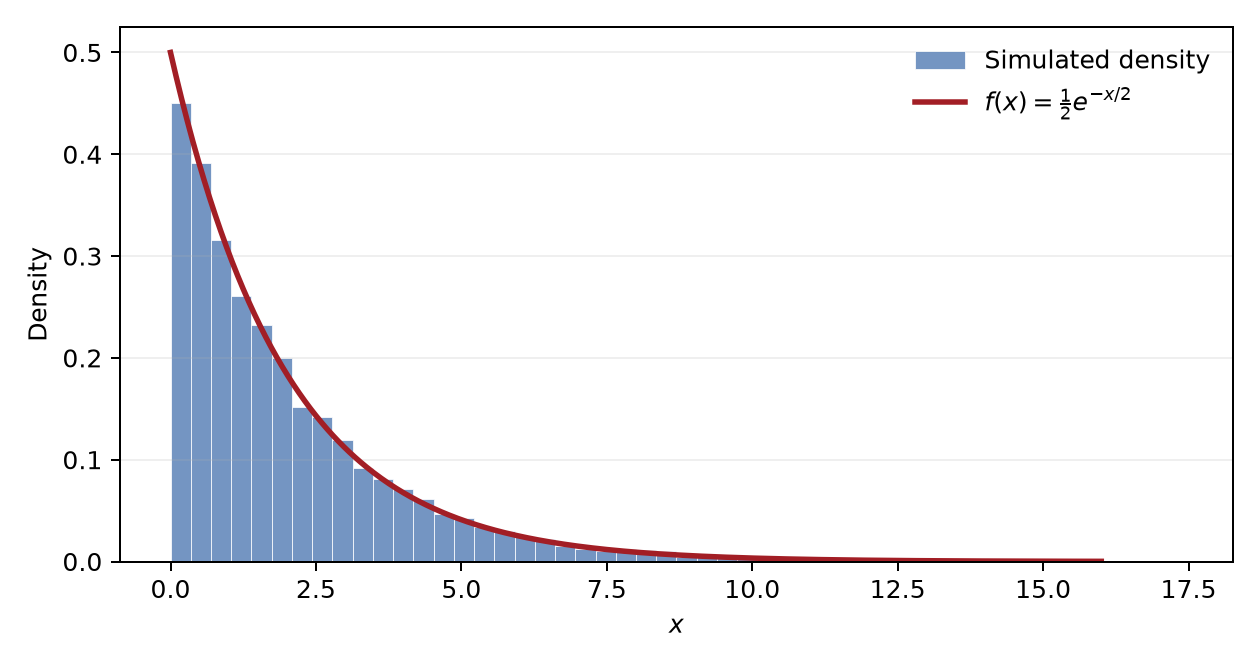
\includegraphics[width=\linewidth]{q2_exponential.png}
\column{0.38\textwidth}
\scriptsize
\setlength{\tabcolsep}{3pt}
\begin{tabular}{lr}
\toprule
Quantity & Value\\\midrule
Sample mean & \QTwoMean\\
Sample variance & \QTwoVariance\\
Theoretical mean & 2\\
Theoretical variance & 4\\\bottomrule
\end{tabular}
\end{columns}
\end{frame}

\begin{frame}{Q2: Inverse transform for the normal distribution}
\small
For $X\sim N(\mu,\sigma^2)$, the PDF is explicit:
\[
f_X(x)=\frac{1}{\sigma\sqrt{2\pi}}
\exp\!\left[-\frac12\left(\frac{x-\mu}{\sigma}\right)^2\right].
\]
Its CDF is defined by integrating this density,
\[
F_X(x)=\int_{-\infty}^x f_X(t)\,dt,
\]
but this integral has no elementary closed-form expression. Numerical methods such as quadrature can approximate $F_X(x)$, and numerical root-finding can then approximate $F_X^{-1}(u)$. In practice, specialized normal quantile algorithms provide this inverse efficiently.
\begin{block}{Takeaway}
Inverse transform sampling applies whenever the CDF can be evaluated and inverted. For the normal distribution, this requires numerical approximations rather than an elementary inverse formula.
\end{block}
\end{frame}

\section[Q3]{Q3: Acceptance--Rejection Sampling}

\begin{frame}{Q3: Problem}
\small
Sample from $f(x)=3x^2$ on $[0,1]$ using acceptance--rejection. Take the proposal density $g(x)=2x$ and
$X'=\sqrt V$ with $V\sim U(0,1)$.
\begin{enumerate}
\item[(a)] Find the smallest constant $\alpha$.
\item[(b)] Simplify $f(X')/(\alpha g(X'))$.
\item[(c)] Give pseudocode for $n$ accepted samples.
\item[(d)] \redstar Produce 10,000 accepted samples and compare with $f$.
\item[(e)] \redstar Compare empirical and theoretical efficiencies.
\end{enumerate}
\end{frame}

\begin{frame}{Q3: Algorithm: Rejection sampling}
\small
To generate samples from a target density $f_X$:
\begin{enumerate}
\item Choose a proposal density $f_Y$ and a finite constant $c$ such that
      $f_X(x)\le c f_Y(x)$ almost everywhere.
\item Draw $Y$ from $f_Y$ and draw $U\sim U(0,1)$ independently.
\item If $U\le \dfrac{f_X(Y)}{c f_Y(Y)}$, return $Y$ as a target sample.
      Otherwise, repeat from step 2.
\end{enumerate}
The acceptance probability is $1/c$. A good proposal is easy to sample,
covers the target support, and makes the smallest possible valid $c$.
\end{frame}

\begin{frame}{Q3(a)--(b): Envelope and acceptance rule}
\small
For $x>0$,
\[
\frac{f(x)}{g(x)}=\frac{3x^2}{2x}=\frac32x,
\qquad
\keybox{\alpha=\sup_{0<x\leq1}\frac{f(x)}{g(x)}=\frac32}.
\]
The ratio at $x=0$ is irrelevant because $P(X'=0)=0$. Consequently,
\[
\frac{f(X')}{\alpha g(X')}
=\frac{3(X')^2}{(3/2)(2X')}=X'.
\]
Draw independent $U,V\sim U(0,1)$, set $X'=\sqrt V$, and
\keytext{accept precisely when $U\leq X'$}.
\medskip
Since $\int f=\int g=1$, the acceptance probability is
\[
P(\text{accept})=\frac1\alpha=\keybox{\frac23}.
\]
\end{frame}

\begin{frame}[fragile]{Q3(c): Pseudocode}
\small
\begin{lstlisting}
accepted = []
proposals = 0
while len(accepted) < n:
    V = Uniform(0, 1)
    U = Uniform(0, 1)  # independent of V
    x_proposal = sqrt(V)
    proposals += 1
    if U <= x_proposal:
        accepted.append(x_proposal)
efficiency = n / proposals
\end{lstlisting}
\end{frame}

\begin{frame}{Q3(d)--(e): Histogram and efficiency}
\footnotesize
\begin{columns}[T]
\column{0.60\textwidth}
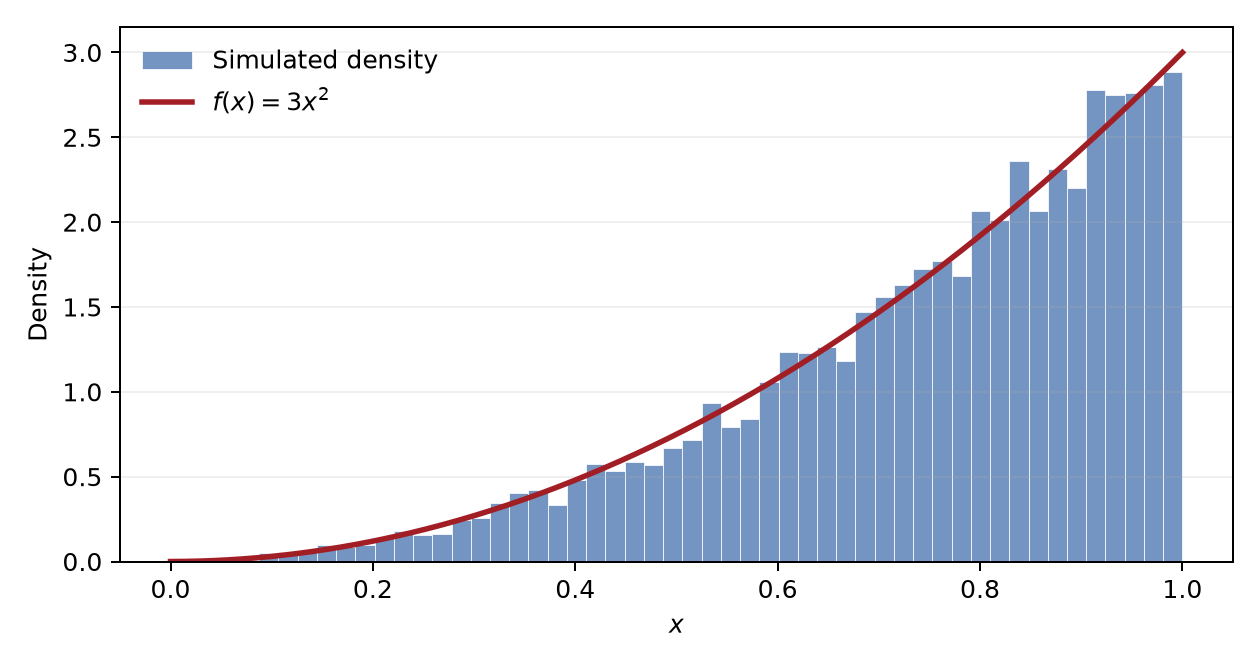
\includegraphics[width=\linewidth]{q3_rejection.png}
\column{0.38\textwidth}
\scriptsize
\setlength{\tabcolsep}{3pt}
\begin{tabular}{lr}
\toprule
Quantity & Value\\\midrule
Accepted samples & 10,000\\
Total proposals & \QThreeProposals\\
Empirical efficiency & \QThreeEfficiency\\
Theoretical efficiency & $2/3$\\\bottomrule
\end{tabular}
\end{columns}
\end{frame}

\begin{frame}{Q3: Example with a beta density}
\small
Consider
\[
f_X(x)=20x(1-x)^3,\qquad 0\le x\le1.
\]
Use the uniform proposal $f_Y(x)=1$ on $[0,1]$. The target is normalized because
\[
\int_0^1 20x(1-x)^3\,dx=1.
\]
The derivative of $f_X$ is $20(1-x)^2(1-4x)$, so its maximum occurs at
$x=1/4$:
\[
c=\max_{[0,1]}\frac{f_X(x)}{f_Y(x)}
=f_X\!\left(\frac14\right)=\frac{135}{64}.
\]
Draw $Y\sim U(0,1)$ and accept when
\[
U\le \frac{20Y(1-Y)^3}{135/64}.
\]
The theoretical acceptance probability is $64/135\approx0.474$.
\end{frame}

\begin{frame}{Q3: Example with a gamma density}
\small
Consider the normalized density
\[
f_X(x)=K\sqrt{x}\,e^{-x},\qquad x\ge0.
\]
Since $\int_0^\infty x^{1/2}e^{-x}\,dx=\Gamma(3/2)=\sqrt\pi/2$,
normalization requires $K=2/\sqrt\pi$. Choose an exponential proposal
with rate $1/2$,
\[
f_Y(x)=\frac12e^{-x/2},\qquad x\ge0.
\]
The density ratio is
\[
\frac{f_X(x)}{f_Y(x)}=\frac4{\sqrt\pi}\sqrt{x}\,e^{-x/2}.
\]
Its maximum occurs at $x=1$, giving $c=4/\sqrt{\pi e}$ and acceptance
probability $1/c=\sqrt{\pi e}/4\approx0.731$. Draw $Y=-2\ln V$ for
$V\sim U(0,1)$ and accept when $U\le f_X(Y)/(c f_Y(Y))$.
\end{frame}

\section[Q4]{Q4: Monte Carlo Integration}

\begin{frame}{Q4: Problem}
\small
Estimate $I=\int_0^1e^{-x^2}\,dx$ by drawing $X_i\sim U(0,1)$.
\begin{enumerate}
\item[(a)] Derive the Monte Carlo estimator.
\item[(b)] \redstar Report estimates for $N=100,1{,}000,10{,}000,100{,}000$.
\item[(c)] \redstar For each $N$, use the sample standard deviation of $e^{-X_i^2}$
to form an approximate 95\% confidence interval.
\item[(d)] \redstar Explain how 95\% CI width changes with $N$.
\end{enumerate}
\end{frame}

\begin{frame}{Q4(a): Integral as an expectation}
\small
The uniform density is one on $[0,1]$, so
\[
I=\int_0^1e^{-x^2}\,dx=\E[e^{-X^2}],
\qquad X\sim U(0,1).
\]
For independent $X_1,\ldots,X_N$, define $H_i=e^{-X_i^2}$ and use
\[
\keybox{\widehat I_N=\frac1N\sum_{i=1}^N H_i},
\qquad
s_H^2=\frac1{N-1}\sum_{i=1}^N(H_i-\widehat I_N)^2.
\]
Then $\E[\widehat I_N]=I$ and the approximate 95\% interval is
$\widehat I_N\pm1.96s_H/\sqrt N$.
\medskip
An independent check is
$I=\frac{\sqrt\pi}{2}\operatorname{erf}(1)=\QFourExact$.
\end{frame}

\begin{frame}{Q4(b)--(c): Estimates and confidence intervals}
\footnotesize
The first $N$ values of one fixed stream are used for each row.
\medskip
\begin{center}
\begin{tabular}{rrrrr}
\toprule
$N$ & $\widehat I_N$ & $s_H$ & 95\% CI lower & 95\% CI upper\\\midrule
100 & \QFourAMean & \QFourASD & \QFourALow & \QFourAHigh\\
1,000 & \QFourBMean & \QFourBSD & \QFourBLow & \QFourBHigh\\
10,000 & \QFourCMean & \QFourCSD & \QFourCLow & \QFourCHigh\\
100,000 & \QFourDMean & \QFourDSD & \QFourDLow & \QFourDHigh\\\bottomrule
\end{tabular}
\end{center}
\medskip
These intervals quantify sampling uncertainty. A particular realized
estimate need not move monotonically toward the true value as $N$ grows.
\end{frame}

\begin{frame}{Q4(d): Why larger $N$ narrows the interval}
\small
For independent $H_i$ with variance $\sigma_H^2$,
\[
\Var(\widehat I_N)=\frac{\sigma_H^2}{N},\qquad
\SE(\widehat I_N)=\frac{\sigma_H}{\sqrt N}.
\]
The approximate full width is $2(1.96)s_H/\sqrt N$.
When $s_H$ stays roughly constant, multiplying $N$ by ten shrinks the
width by about $1/\sqrt{10}\approx0.316$; multiplying $N$ by 100
shrinks it by about $1/10$.
\end{frame}

\section[Q5]{Q5: Monte Carlo Call Pricing}

\begin{frame}{Q5: Problem}
\small
Under the risk-neutral Black--Scholes model, let
\[
S_T=S_0\exp\!\left((r-\tfrac12\sigma^2)T+\sigma\sqrt T Z\right),
\quad Z\sim N(0,1),
\]
with $S_0=95$, $K=100$, $r=0.01$, $\sigma=0.4$, $T=1$.
The European call price is $c_0=e^{-rT}\E[(S_T-K)^+]$.
\begin{enumerate}
\item[(a)] Derive the crude Monte Carlo estimator.
\item[(b)] \redstar Estimate the option price using N= 10,000 simulations.
\item[(c)] \redstar Construct a 95\% CI for the option price.
\item[(d)] \redstar Repeat with $N=100{,}000$ and compare.
\item[(e)] \redstar Explain the $N^{-1/2}$ standard-error scaling.
\end{enumerate}
\end{frame}

\begin{frame}{Q5(a): Discount each simulated payoff}
\small
For independent $Z_i\sim N(0,1)$, compute
\[
S_T^{(i)}=95\exp(-0.07+0.4Z_i),\qquad
W_i=e^{-0.01}(S_T^{(i)}-100)^+.
\]
Then
\[
\keybox{\widehat c_N=\frac1N\sum_{i=1}^N H_i
=e^{-rT}\frac1N\sum_{i=1}^N(S_T^{(i)}-K)^+}.
\]
The estimated standard error is $s_H/\sqrt N$, where $s_H$ is the sample
standard deviation of the \emph{discounted} payoffs. Hence the 95\%
interval is $\widehat c_N\pm1.96s_H/\sqrt N$.
\end{frame}

\begin{frame}{Q5(b)--(d): Numerical call estimates}
\footnotesize
The 10,000-path run is the prefix of the 100,000-path run.
\medskip
\begin{center}
\begin{tabular}{rrrrr}
\toprule
$N$ & Estimate & Estimated SE & 95\% CI lower & 95\% CI upper\\\midrule
10,000 & \QFiveAMean & \QFiveASE & \QFiveALow & \QFiveAHigh\\
100,000 & \QFiveBMean & \QFiveBSE & \QFiveBLow & \QFiveBHigh\\\bottomrule
\end{tabular}
\end{center}
\medskip
The Black--Scholes closed-form price, used only as a check, is
$c_0=\QFiveExact$. Both Monte Carlo intervals contain this value.
The 100,000-path interval is narrower and its estimate happens to be
closer to the check value; a larger $N$ does not guarantee that the
realized error decreases on every run.
\end{frame}

\begin{frame}{Q5(e): Error Scaling}
\small
Since $\Var(\widehat c_N)=\Var(H)/N$,
\[
\SE(\widehat c_{100N})=\frac1{10}\SE(\widehat c_N)
\quad\text{when the payoff variance is fixed.}
\]
Thus reducing standard error by a factor of 10 generally requires
\keytext{100 times as many paths}.
\end{frame}

\section[Q6]{Q6: Antithetic Variates}

\begin{frame}{Q6: Problem}
\small
Use the parameters of Q5 and 10,000 independent base draws $Z_i$.
For each, form a pair $Z_i,-Z_i$ and terminal prices $S_T^+,S_T^-$.
\begin{enumerate}
\item[(a)] Explain why $Z$ and $-Z$ have the same law.
\item[(b)] Implement the antithetic variates estimator.
\item[(c)] \redstar Compute the estimated option price and a 95\% CI.
\item[(d)] \redstar Compare its standard error with crude Monte Carlo.
\end{enumerate}
\end{frame}

\begin{frame}{Q6: Algorithm: Antithetic variates}
\small
To estimate $\theta=\E[h(X)]$:
\begin{enumerate}
\item Generate $N$ independent pairs $(X_i,X_i')$ with the same marginal
      distribution as $X$, chosen so that $h(X_i)$ and $h(X_i')$ are negatively
      correlated. Common examples are $(U_i,1-U_i)$ for uniform draws and
      $(Z_i,-Z_i)$ for standard normal draws.
\item Form the pair averages
      $A_i=\tfrac12[h(X_i)+h(X_i')]$ and estimate
      $\theta$ by $\widehat\theta_{\rm AV}=\mu_{A,N}$.
\item Estimate the standard error using the sample standard deviation of the
      $N$ pair averages divided by $\sqrt N$. Form a 95\% confidence interval
      as the estimate plus or minus 1.96 times this estimated standard error.
\end{enumerate}
If each payoff has variance $\sigma_H^2$ and within-pair correlation $\rho$,
then $\sigma_A^2=\sigma_H^2(1+\rho)/2$. Negative correlation reduces variance.
\end{frame}

\begin{frame}{Q6(a)--(b): Antithetic variates estimator}
\small
The standard normal density satisfies $\phi(-z)=\phi(z)$, so
$Z\stackrel{d}{=}-Z$. For each $Z_i$, define
\[
S_{T,i}^{\pm}=95\exp(-0.07\pm0.4Z_i),\qquad
A_i=\frac{e^{-0.01}}2
\left[(S_{T,i}^+-100)^++(S_{T,i}^--100)^+\right].
\]
Then the antithetic estimate is $\widehat c_{\rm AV}=N^{-1}\sum_iA_i$.
Each $A_i$ has expectation $c_0$, and pairs are independent across $i$.
The two payoffs \emph{within} a pair are dependent.
\[
\keybox{\widehat{\SE}_{\rm AV}=\frac{s_A}{\sqrt N}}
\]
Use the sample standard deviation of the \emph{10,000 pair averages},
not the standard deviation of 20,000 individual payoffs divided by $\sqrt{20,000}$.
\end{frame}

\begin{frame}{Q6(c)--(d): Price and standard error}
\footnotesize
\begin{center}
\begin{tabular}{lrrrr}
\toprule
Method & Estimate & Estimated SE & 95\% lower & 95\% upper\\\midrule
Crude Q5, 10,000 paths & \QFiveAMean & \QFiveASE & \QFiveALow & \QFiveAHigh\\
Crude, same 10,000 $Z_i$ & \QSixCrudeMean & \QSixCrudeSE & \QSixCrudeLow & \QSixCrudeHigh\\
Antithetic, 10,000 pairs & \QSixAVMean & \QSixAVSE & \QSixAVLow & \QSixAVHigh\\\bottomrule
\end{tabular}
\end{center}
\medskip
The antithetic standard error is smaller in this run. The same-$Z_i$
crude row isolates the pairing effect; the Q5 row matches the comparison
requested in the assignment. A pair evaluates two payoffs, so a
\emph{fixed-computational-cost} comparison would also compare against
20,000 independent crude paths.
\end{frame}

\begin{frame}{Q6: Why pairing can reduce variance}
\small
Let $P^+=e^{-rT}(S_T^+-K)^+$ and
$P^-=e^{-rT}(S_T^--K)^+$. They have the same variance $\sigma_P^2$.
For the pair average $A=(P^++P^-)/2$,
\[
\Var(A)=\frac{\sigma_P^2}{2}
\left(1+\operatorname{Corr}(P^+,P^-)\right).
\]
The call payoff is nondecreasing in $Z$, whereas its paired payoff is
nonincreasing in $Z$, so their covariance is nonpositive. This makes
the pair average less variable than a single crude payoff, and often
less variable than the average of two independent payoffs.
\end{frame}

\section[Q7]{Q7: Control Variates}

\begin{frame}{Q7: Problem}
\small
Let $X\sim\operatorname{Exp}(1)$, $H=X^{0.9}$, and choose the control
$Y=X$, for which $\E[Y]=1$. Define
\[
H^*=X^{0.9}+c(X-1),
\qquad c^*=-\frac{\Cov(X^{0.9},X)}{\Var(X)}.
\]
\begin{enumerate}
\item[(a)] \redstar Generate 10,000 samples from $X\sim \operatorname{Exp}(1)$.
\item[(b)] \redstar Estimate $\E[X^{0.9}]$ using crude Monte Carlo.
\item[(c)] \redstar Estimate $c^*$ using sample covariance and variance.
\item[(d)] \redstar Give the control variate estimator.
\item[(e)] \redstar Compare sample standard deviations.
\end{enumerate}
\end{frame}

\begin{frame}{Q7: Algorithm: Control variates}
\small
To estimate $\theta=\E[H]$, choose a variable $Y$ from the same simulation
with known mean $\mu_Y=\E[Y]$ and strong correlation with $H$.
\begin{enumerate}
\item Generate independent pairs $(H_i,Y_i)$.
\item Choose a coefficient $c$. The variance-minimizing value is
      $c^*=-\Cov(H,Y)/\sigma_Y^2$. If the covariance and variance are unknown,
      estimate them from the simulated sample.
\item Form $H_i^*=H_i+c(Y_i-\mu_Y)$ and estimate $\theta$ by their sample mean
      $\widehat\theta_{\rm CV}=\mu_{H^*,N}$. Estimate its standard error from
      the sample standard deviation of $H_i^*$ divided by $\sqrt N$.
\end{enumerate}
For fixed $c$, $\E[H_i^*]=\E[H]$. At $c=c^*$,
$\sigma_{H^*}^2=\sigma_H^2(1-\rho_{H,Y}^2)$.
\end{frame}

\begin{frame}{Q7(a)--(d): Both estimators from the same samples}
\small
Generate independent $U_i\sim U(0,1)$ and set
$X_i=-\ln(1-U_i)$, $H_i=X_i^{0.9}$, $Y_i=X_i$.
The crude estimator is $\bar H$.
\[
\widehat c=-\frac{\sum_i(H_i-\bar H)(Y_i-\bar Y)}
{\sum_i(Y_i-\bar Y)^2},
\qquad
\keybox{\widehat\theta_{\rm CV}
=\frac1N\sum_i\left[H_i+\widehat c(Y_i-1)\right]}.
\]
For this fixed sample, $\widehat c=\QSevenCoeff$.
The resulting means are $\bar H=\QSevenCrudeMean$ and
$\widehat\theta_{\rm CV}=\QSevenCVMean$.
\medskip
An exact benchmark is $\E[X^{0.9}]=\Gamma(1.9)=\QSevenExact$.
\end{frame}

\begin{frame}{Q7(e): Variance reduction and exact coefficient}
\footnotesize
\begin{center}
\begin{tabular}{lrrr}
\toprule
Method & Mean estimate & Sample SD of values & Estimated SE\\\midrule
Crude $H_i$ & \QSevenCrudeMean & \QSevenCrudeSD & \QSevenCrudeSE\\
Control $H_i+\widehat c(Y_i-1)$ & \QSevenCVMean & \QSevenCVSD & \QSevenCVSE\\\bottomrule
\end{tabular}
\end{center}
\medskip
The adjusted sample values have a much smaller standard deviation.
For an analytic cross-check, $\E[X^p]=\Gamma(p+1)$,
$\Var(X)=1$, and
\[
\Cov(X^{0.9},X)
=\Gamma(2.9)-\Gamma(1.9)=0.9\Gamma(1.9),
\quad c^*=-0.9\Gamma(1.9)=\QSevenExactCoeff.
\]
The sample coefficient is close to this optimum. Because $\widehat c$
is fitted on the same sample, the exact fixed-$c$ unbiasedness statement
does not apply literally at finite $N$; the effect is small here.
\end{frame}

\section*{End}

\begin{frame}{}
\centering
\vfill
{\Huge\color{blue!70!black}\textbf{Thank You!}}
\vspace{1cm}
{\Large Questions?}
\vfill
\end{frame}

\end{document}
